\chapter[Hypothesis Tests]{Hypothesis Tests: Errors, Level, Power and $p$-Values}
\label{ch:tests-foundations}

\begin{chaptergoals}
\begin{itemize}[nosep]
\item What a test is: a yes/no rule applied to the data, written as an indicator of a rejection region. The null hypothesis is the claim the data are allowed to overturn; the alternative is what you conclude when they do.
\item The two ways a test can be wrong, why they are not treated alike, and the two numbers that describe a test: its level, a cap on one error, and its power, one minus the other.
\item The recipe behind every test in this book: a test statistic whose distribution under the null hypothesis you know, and a quantile of that distribution as the threshold. One-sided and two-sided versions, and why the null hypothesis makes the unknown parameter known.
\item The test for the kiss data, done exactly and done by the CLT: thresholds $72$ and $74$ one way, $72$ and $73$ the other, and why they differ.
\item The $p$-value: the smallest level at which the data reject, and the one number a test reports.
\item Tests and confidence intervals are the same construction seen from two sides.
\end{itemize}
The running example is the kiss experiment: $n = 124$ couples, $80$ turning right, and the question \cref{ch:kiss} opened with, whether $80$ is more than chance would produce if couples had no preference for either side.
\end{chaptergoals}

\section{A yes/no question about a parameter}
\label{sec:tests-question}

A confidence interval reports a range.
Often what is wanted is a decision.
The examples below are the kind a manager or a scientist actually faces, and each is a yes/no question about a parameter of a model.

\begin{itemize}
\item \textbf{Boarding a plane.} Two airlines board differently: one from the rear of the plane to the front (`R2F'), the other by window seats first, then middle, then aisle (`WilMA').
Which is faster?
The data are $n = 72$ R2F flights averaging $24.2$ minutes with a standard deviation of $2.1$, and $m = 56$ WilMA flights averaging $15.9$ minutes with a standard deviation of $1.3$.
With boarding times modeled as $X \sim \Gauss(\mu_1, \sigma_1^2)$ and $Y \sim \Gauss(\mu_2, \sigma_2^2)$ and the two samples independent, the question is: is $\mu_1 = \mu_2$, or is $\mu_1 > \mu_2$?
Two samples, one question: a \textbf{two-sample test}.
\item \textbf{Waiting in the emergency room.} The national average wait is $30$ minutes.
Patients at one hospital say its wait is longer.
With $\Xton$ the waits of $n$ random patients there and $\mu = \E[X_1]$, the question is: is $\mu > 30$?
One sample: a \textbf{one-sample test}.
\item \textbf{The kiss experiment.} If couples have no preference for either side, $p = \frac12$.
Of $124$ couples, $80$ turned right.
Is $p = \frac12$, or not?
\end{itemize}

The obvious first answer to the boarding question is `$\bar{X}_n = 24.2 > 15.9 = \bar{Y}_m$, so $\mu_1 > \mu_2$'.
What is wrong with it is this: by bad luck the $72$ R2F flights might all have been full and the $56$ WilMA flights half empty, and sample means move from sample to sample.
A better rule puts a buffer around each mean and asks whether the buffers still separate:
\[
\text{conclude } \mu_1 > \mu_2 \text{ if } \bar{X}_n - \text{buffer} > \bar{Y}_m + \text{buffer}.
\]
For the one-sample version, conclude $\mu > 30$ if $\bar{X}_n > 30 + \text{buffer}$.
What should the buffer be?
Something that measures the size of the random fluctuations of $\bar{X}_n$, and \cref{ch:clt} says what that is: a few multiples of $\sigma/\sqrt{n}$.
\Cref{fig:testbuffer} draws the heuristic for the boarding data and for two one-sample examples, with a buffer of two standard errors around each estimate.
With $n = 72$ and $m = 56$ the buffers around $24.2$ and $15.9$ minutes reach about half a minute (R2F) and a third of a minute (WilMA) on each side, nowhere near each other, and the conclusion is not in doubt.
For a coin tossed $30$ times with $13$ heads, the buffer $0.43 \pm 0.18$ reaches well past $\frac12$, and the heuristic says nothing.
For a survey of $4{,}971$ Americans in which $32\%$ get news on YouTube, the buffer $0.32 \pm 0.013$ just reaches the $33\%$ being tested, and again the heuristic is silent.
For a proportion the buffer is $2\sqrt{\hat{p}(1-\hat{p})/n}$, and it shrinks like $1/\sqrt{n}$.

\begin{figure}[htbp]
\centering
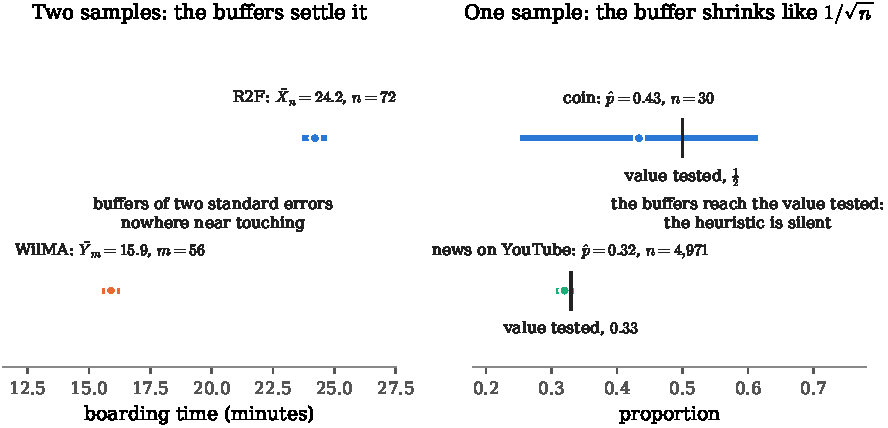
\includegraphics[width=\textwidth]{fig_test_buffer}
\caption{Buffers of two standard errors around each estimate (dot). Left: the boarding data, R2F (blue) and WilMA (orange). Right: two one-sample proportions, the coin (blue) and the YouTube survey (aqua), each with the value being tested as a black tick.}
\label{fig:testbuffer}
\end{figure}

The rest of the chapter makes the heuristic precise: what counts as a buffer, what guarantee it comes with, and what to report when the data land near the edge.

\begin{bridge}[statistically significant]
Every one of these questions was answered in an introductory course with a $z$-test or a $t$-test and the phrase `the difference is statistically significant at the $5\%$ level'.
This chapter is that procedure, written so that each piece has a name and a guarantee: the hypotheses, the rejection region, the two errors, the level, the power and the $p$-value.
`Significant at $5\%$' will turn out to mean `the test of level $5\%$ rejected', and `$p < 0.05$' will be a theorem rather than a rule of thumb.
\end{bridge}

\section{Null and alternative hypotheses}
\label{sec:tests-hypotheses}

Let $\Xton$ be a sample of i.i.d.\ r.v.s and $\statmodel$ a statistical model (\cref{ch:models}).
Let $\Theta_0$ and $\Theta_1$ be disjoint subsets of $\Theta$.
The two hypotheses are
\[
H_0: \theta \in \Theta_0 \qquad \text{and} \qquad H_1: \theta \in \Theta_1.
\]
$H_0$ is the \textbf{null hypothesis}, $H_1$ the \textbf{alternative hypothesis}.
If you believe the true $\theta$ is in one of the two sets, you test $H_0$ against $H_1$: you look in the data for evidence against $H_0$, and you decide whether to \textbf{reject} $H_0$.\footnote{Some treatments require $\Theta_0$ and $\Theta_1$ to partition $\Theta$, and others, this book among them, ask only that the two sets be disjoint. The difference matters when values of $\theta$ in neither set are possible, in which case the test is silent about them. In every example in this book the two sets partition $\Theta$.}

The two hypotheses do not play symmetric roles, and this asymmetry is the first thing to internalize.
The data are used only to try to disprove $H_0$.
If they fail to, that is not evidence that $H_0$ is true; it is a lack of evidence against it.
The standard phrase is `innocent until proven guilty': the null hypothesis is the defendant, the data are the evidence, and a verdict of not guilty is not a finding of innocence.
So the conclusions of a test are `reject $H_0$' and `fail to reject $H_0$', never `accept $H_0$'.

Which claim goes in the null?
The one that gets the benefit of the doubt: the status quo, the claim of no effect, the value you would act on if the data said nothing.
For the kiss experiment the null is $p = \frac12$, no preference; for the emergency room it is `the wait is not longer than the national average'; for the boarding methods it is `no difference'.
The alternative is the claim that needs evidence to be adopted, and it is the one the study was run to look for.

\textbf{Simple and composite.}
A hypothesis is \textbf{simple} if its set is a single point, $\Theta_k = \{\theta_k\}$, and \textbf{composite} otherwise, typically a half-line $\{\theta > \theta_k\}$ or $\{\theta < \theta_k\}$ or everything but a point, $\{\theta \neq \theta_k\}$.
When $\Theta \subseteq \real$ and $H_0$ is simple, $H_0: \theta = \theta_0$, the terminology is:
\begin{itemize}[nosep]
\item \textbf{two-sided test}: $H_1: \theta \neq \theta_0$, departures in either direction count as evidence;
\item \textbf{one-sided test}: $H_1: \theta > \theta_0$ or $H_1: \theta < \theta_0$, only one direction counts.
\end{itemize}
One-sided tests are also written with a composite null, $H_0: \theta \leq \theta_0$ against $H_1: \theta > \theta_0$; \cref{sec:tests-errors} explains why the two forms of the null lead to the same test.
For the examples above: the boarding question is one-sided ($\mu_1 > \mu_2$); the emergency room is one-sided ($\mu > 30$); the fair coin is two-sided ($p \neq \frac12$); and the test for the kiss data can be put either way, two-sided as $H_0: p = \frac12$ against $H_1: p \neq \frac12$, or one-sided as \cref{ch:kiss} asked it, $H_1: p > \frac12$.
Both are done below.

\begin{pitfall}[one-sided is a modeling decision, not a reading of the data]
Writing $H_1: \mu_1 > \mu_2$ for the boarding methods says that $\mu_1 < \mu_2$ is not a possibility you entertain.
The modeling assumption reduces the number of ways the hypothesis $\mu_1 = \mu_2$ can be rejected: $\mu_1 < \mu_2$ is not allowed, so a sample pointing that way counts as no evidence against the null at all.
That decision has to be made before looking at the data.
Choosing the side after seeing which way $\bar{X}_n - \bar{Y}_m$ came out is a way of rejecting more often than the level promises: a nominal $5\%$ becomes an actual $10\%$, since a two-sided question is then being answered with a one-sided threshold.
\Cref{sec:tests-kiss} shows the thresholds differ ($72$ against $74$ right turns for the kiss data), which is exactly the room this mistake exploits.
\end{pitfall}

\section{What a test is}
\label{sec:tests-definition}

\begin{definition}[Test, rejection region]
\label{def:test}
A \textbf{test} is a statistic $\psi: E^n \to \{0, 1\}$: a function of the sample $\Xton$ taking the values $0$ and $1$, such that
\begin{itemize}[nosep]
\item if $\psi(\Xton) = 0$, $H_0$ is not rejected;
\item if $\psi(\Xton) = 1$, $H_0$ is rejected.
\end{itemize}
The \textbf{rejection region} of $\psi$ is the set of samples on which it rejects,
\[
R_\psi = \{ (x_1, \ldots, x_n) \in E^n : \psi(x_1, \ldots, x_n) = 1 \},
\]
so that $\psi = \ind(R_\psi)$ \toolkit{sec:math-indicator}.
\end{definition}

\begin{inwords}
\textbf{In words.} A test is a rule, fixed before the data arrive, that sorts every possible sample into two bins: reject or don't. The rejection region is the `reject' bin, and the test is its indicator. Because the rule is applied to a random sample, $\psi$ is a random variable, a Bernoulli one, and asking how often it equals $1$ is a probability question, like asking how often an interval covers.
\par\smallskip
\textbf{For the kiss data.} `Reject $p = \frac12$ if $72$ or more of the $124$ couples turn right' is the test $\psi = \ind(n\bar{R}_n \geq 72)$. Its rejection region is every sequence of $124$ zeros and ones with at least $72$ ones. On the sample we have, $n\bar{R}_n = 80$ and $\psi = 1$.
\end{inwords}

The definition contains no probability: a test is a partition of the sample space $E^n$ of \cref{sec:models-sample-space} into two pieces.
Probability enters when you ask how the test behaves under each candidate $\Pr_\theta$, which is the next section.

In practice every test in this book has the form
\[
\psi = \ind( T_n > c )
\]
for a statistic $T_n = T_n(\Xton)$, called the \textbf{test statistic}, and a number $c$, the \textbf{threshold}; the rejection region is then $\{T_n > c\}$ (for a count, `$\geq 72$' is `$> 71$', so the strict inequality is only a matter of where $c$ sits).
The test statistic compresses the sample into one number that measures how far the data are from what $H_0$ predicts, and the threshold says how far is too far.
Everything a test does is in those two choices, and the sections that follow are about making them.

\begin{bridge}[the test statistic you already know]
In an introductory course the test statistic was $z = (\bar{x} - \mu_0)/(\sigma/\sqrt{n})$, or $t$ with $s$ in place of $\sigma$, and the threshold was a number from a table, $1.96$ or $1.645$ or a $t$ critical value.
That is $\psi = \ind(\abs{T_n} > c)$ with $T_n$ the standardized mean.
What this chapter adds is the function $\psi$ itself as an object, so that `the test rejects with probability $\alpha$ when $H_0$ is true' is a statement about a random variable with a definition, and so that tests with other statistics (likelihood ratios in \cref{ch:wald-lrt}, chi-squared distances in \cref{ch:gof}) are the same object with a different $T_n$.
\end{bridge}

\section{Two kinds of error, level and power}
\label{sec:tests-errors}

A test can be wrong in two ways, and the standard table lays them out with the truth in the rows and the decision in the columns:
\begin{center}
\begin{tabular}{@{}lcc@{}}
\toprule
 & not rejected ($\psi = 0$) & rejected ($\psi = 1$) \\
\midrule
$H_0$ true ($\theta \in \Theta_0$) & correct & \textbf{type 1 error} \\
$H_1$ true ($\theta \in \Theta_1$) & \textbf{type 2 error} & correct \\
\bottomrule
\end{tabular}
\end{center}
A \textbf{type 1 error} is rejecting $H_0$ when it is true: convicting the innocent.
A \textbf{type 2 error} is failing to reject $H_0$ when $H_1$ is true: acquitting the guilty.
Since the truth is one fixed $\theta$ and the decision is random, the natural measure of each error is a probability, and since the probability depends on which $\theta$ is true, each error is a \textit{function} of $\theta$ on its own hypothesis.

\begin{definition}[Type 1 error, type 2 error, power]
\label{def:errors}
For a test $\psi$ of $H_0: \theta \in \Theta_0$ against $H_1: \theta \in \Theta_1$:
\begin{itemize}[nosep]
\item the \textbf{type 1 error} of $\psi$ is the function
\[
\alpha_\psi: \Theta_0 \to [0, 1], \qquad \theta \mapsto \Pr_\theta(\psi = 1);
\]
\item the \textbf{type 2 error} of $\psi$ is the function
\[
\beta_\psi: \Theta_1 \to [0, 1], \qquad \theta \mapsto \Pr_\theta(\psi = 0);
\]
\item the \textbf{power} of $\psi$ is the number \toolkit{sec:math-sup}
\[
\pi_\psi = \inf_{\theta \in \Theta_1} \left( 1 - \beta_\psi(\theta) \right).
\]
\end{itemize}
\end{definition}

\begin{inwords}
\textbf{In words.} Fix a truth $\theta$ and imagine rerunning the study many times. If $\theta$ is in the null set, the fraction of reruns on which the test rejects is the type 1 error at that $\theta$; if $\theta$ is in the alternative, the fraction on which it fails to reject is the type 2 error at that $\theta$, and the fraction on which it rejects is the power at that $\theta$. The power of the test is the worst case of that last fraction over the whole alternative: the least the test can be relied on to detect a departure from $H_0$.
\par\smallskip
\textbf{For the kiss data.} For $\psi = \ind(n\bar{R}_n \geq 72)$ and the one-sided hypotheses $H_0: p = \frac12$, $H_1: p > \frac12$: the type 1 error is the single number $\Pr_{1/2}(n\bar{R}_n \geq 72) = 0.044$. The type 2 error at $p = 0.645$ is $\Pr_{0.645}(n\bar{R}_n \leq 71) = 0.057$, so the test detects a true $p$ of $0.645$ with probability $0.943$. The power in the definition's sense is $\inf_{p > 1/2}$ of that detection probability, which is $0.044$, approached as $p \downarrow \frac12$: no test can reliably detect a $p$ just above $\frac12$ with $124$ couples, and the infimum records that.
\end{inwords}

\begin{figure}[htbp]
\centering
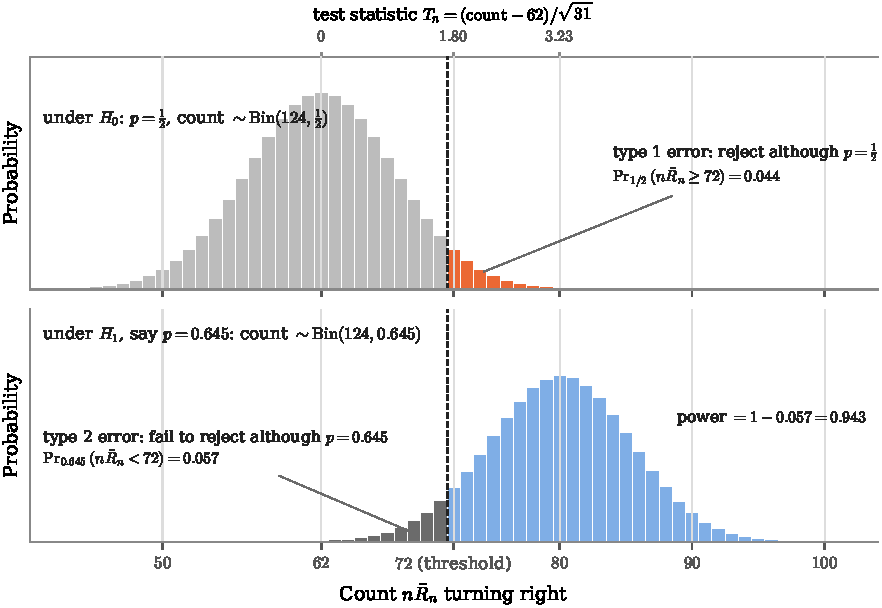
\includegraphics[width=\textwidth]{fig_test_two_errors}
\caption{The test `reject $p = \frac12$ if the count is $72$ or more', threshold dashed. Top: the count under $p = \frac12$, mass at $72$ and above in orange. Bottom: the count under $p = 0.645$, mass below $72$ in gray, the rest in blue.}
\label{fig:twoerrors}
\end{figure}

\Cref{fig:twoerrors} is the picture to hold on to.
The same threshold cuts two different distributions of the count: the one $H_0$ predicts and one of the many $H_1$ allows.
At the top, if $p = \frac12$ the count is $\mathrm{Bin}(124, \frac12)$, centered at $62$, and the orange mass at $72$ and above is the type 1 error, $0.044$.
At the bottom, if instead $p = 0.645$ the count is $\mathrm{Bin}(124, 0.645)$, centered at $80$; the gray mass below $72$ is the type 2 error at that $p$, $0.057$, and the blue mass is the power there, $0.943$.
What falls on the wrong side of the cut under each is the corresponding error.
The scale along the top of each is the test statistic $T_n = (\text{count} - 62)/\sqrt{31}$ of \cref{sec:tests-clt}: the threshold $72$ is $T_n = 1.80$, and the observed $80$ is $3.23$.
And the picture shows the trade: sliding the threshold to the right makes the type 1 error smaller and the type 2 error larger (the orange shrinks and the gray grows), sliding it left does the reverse, and at a fixed $n$ you cannot shrink both.
The two distributions pull apart as $n$ grows (their standard deviations are $\sqrt{p(1-p)/n}$ on the proportion scale), and that is the only lever that lowers both errors at once.

Rather than two functions on two sets, it is often clearer to look at one function on all of $\Theta$, the probability of rejecting,
\[
\theta \mapsto \Pr_\theta(\psi = 1),
\]
which is $\alpha_\psi$ on $\Theta_0$ and $1 - \beta_\psi$ on $\Theta_1$.\footnote{Two conventions for the letter $\beta$ are in common use. This book writes $\beta_\psi$ for the type 2 error, as in \cref{def:errors}. Elsewhere $\beta(\theta)$ names this rejection probability itself, the power function, which is $1 - \beta_\psi(\theta)$ on $\Theta_1$ and $\alpha_\psi(\theta)$ on $\Theta_0$. Check which one a source means before carrying a formula across.}
\Cref{fig:powercurve} draws it for the kiss data, computed exactly from the Binomial distribution of the count.
On the left, at $n = 124$, the one-sided test rejects for a count of $72$ or more and the two-sided test for $74$ or more or $50$ or fewer.
At $p = \frac12$ both curves are at or below $0.05$ (they are $0.044$ and $0.038$); to the right both climb to $1$, the one-sided test faster since it spends its whole $5\%$ on that side; to the left the two-sided test climbs and the one-sided test, which does not watch that side, stays at $0$.
On the right, the one-sided test at $n = 30$ (threshold $20$) sits beside the same test at $n = 124$: more data makes the curve steeper, so both errors fall at once.
A good test has a rejection curve that is low on $\Theta_0$ and climbs quickly to $1$ on $\Theta_1$; the level, defined next, caps the low part, and the power is the lowest point of the high part.

\begin{figure}[htbp]
\centering
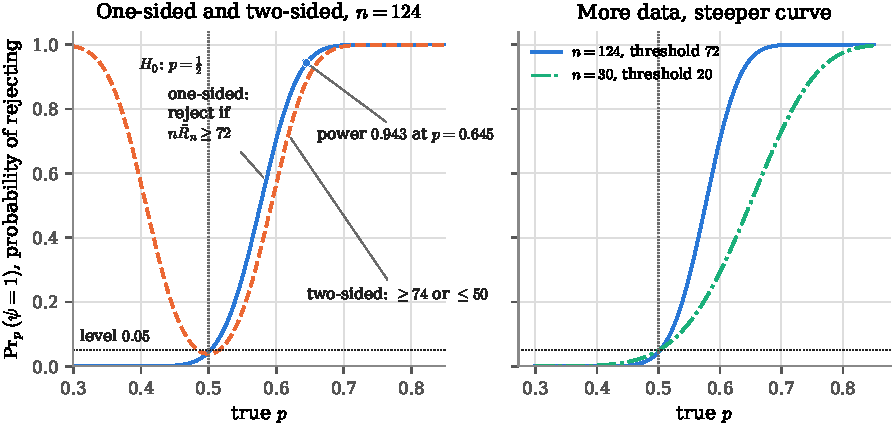
\includegraphics[width=\textwidth]{fig_power_curve}
\caption{The probability of rejecting against the true $p$, with the level $0.05$ dotted. Left, $n = 124$: one-sided, count $\geq 72$ (solid), and two-sided, $\geq 74$ or $\leq 50$ (dashed). Right: one-sided at $n = 124$ (solid) and $n = 30$ (dash-dot).}
\label{fig:powercurve}
\end{figure}

\begin{bridge}[$\alpha$, $\beta$ and the power calculation]
An introductory course calls the type 1 error probability $\alpha$ and the type 2 error probability $\beta$, says `power $= 1 - \beta$', and may have made you compute the sample size needed for $80\%$ power against a specific alternative.
All of that is here. The only addition is that $\alpha$ and $\beta$ are functions of $\theta$, not single numbers: a type 2 error of $0.057$ is a type 2 error \textit{at} $p = 0.645$, and at $p = 0.55$ the same test has a type 2 error of $0.72$, which is why failing to reject is not accepting: this test misses a true $p$ of $0.55$ nearly three times in four.
The power calculation of an introductory course picks one alternative and reads one point off \cref{fig:powercurve}'s curve; the power $\pi_\psi$ of \cref{def:errors} takes the infimum over all of them, which for a composite alternative that touches $\Theta_0$ is the rejection probability at the edge of $\Theta_0$, $0.044$ here: at most the level, and useless as a summary of what the test can detect. The one-point version is the useful one in planning a study, and the infimum is the one that describes the test over the whole alternative.
\end{bridge}

\begin{definition}[Level, asymptotic level]
\label{def:level}
Let $\alpha \in (0, 1)$.
A test $\psi$ has \textbf{level} $\alpha$ if
\[
\alpha_\psi(\theta) \leq \alpha \quad \text{for all } \theta \in \Theta_0,
\]
and \textbf{asymptotic level} $\alpha$ if
\[
\limn \alpha_{\psi_n}(\theta) \leq \alpha \quad \text{for all } \theta \in \Theta_0,
\]
where $\psi_n$ is the test built on $n$ observations \toolkit{sec:math-limits}.
\end{definition}

\begin{inwords}
\textbf{In words.} A test of level $5\%$ is one that convicts the innocent at most $5\%$ of the time, whichever innocent $\theta$ is the truth. The level is a cap on the worst case of the type 1 error over the whole null set, not the type 1 error at one point. `Asymptotic' means the cap is guaranteed only in the limit of large samples, which is what a CLT-based threshold delivers.
\par\smallskip
\textbf{For the kiss data.} $\psi = \ind(n\bar{R}_n \geq 72)$ has level $5\%$ for $H_0: p = \frac12$ exactly, since $0.044 \leq 0.05$; it also has level $5\%$ for the composite null $H_0: p \leq \frac12$, since $\Pr_p(n\bar{R}_n \geq 72)$ only decreases as $p$ falls below $\frac12$. The threshold $71$ would not do: $\Pr_{1/2}(n\bar{R}_n \geq 71) = 0.063$.
\end{inwords}

Two remarks on the definition, both consequences of the asymmetry of \cref{sec:tests-hypotheses}.
First, the level is a guarantee about the type 1 error only.
A test of level $5\%$ promises nothing about its type 2 error; $\psi \equiv 0$, the test that never rejects, has level $5\%$ (its type 1 error is $0$) and is useless.
The standard way of choosing a test is to fix the level first and then, among tests of that level, prefer the one with the most power.
Second, the level is a cap, so a test of level $5\%$ is also a test of level $10\%$: `level $5\%$' is a one-directional bound, as `level $95\%$' was for an interval in \cref{ch:confidence-intervals}, the worst the procedure can do rather than what it does.

\begin{pitfall}[level $\alpha$ for a test, level $1 - \alpha$ for an interval]
The same word, the same $\alpha$, complementary conventions.
For a confidence interval the level is $1 - \alpha$, the probability of a correct capture.
For a test the level is $\alpha$, the probability of an incorrect rejection.
Both conventions describe the procedure by the guarantee it gives, and the guarantee for a test is about the error it controls.
\Cref{sec:tests-duality} shows the two procedures are one object, which is why the same $\alpha$ appears in both.
\end{pitfall}

\begin{intuition}[why the worst case over $\Theta_0$]
For a one-sided question such as `can we conclude that at most a third of Americans get news on YouTube?' you would write $H_0: p \geq 0.33$ against $H_1: p < 0.33$, a composite null. Which $p$ in $\Theta_0$ should the threshold be computed from?
The definition answers: the one that makes rejection most likely, since the level must hold for every $p$ in $\Theta_0$.
The test rejects when $\hat{p}$ is small, and a small $\hat{p}$ is likeliest when $p$ is as small as $\Theta_0$ allows, that is, at the boundary $p = 0.33$.
So the composite null $p \geq 0.33$ is tested with the threshold of the simple null $p = 0.33$, and no separate computation is needed.
The same reasoning gives the threshold $72$ of the kiss data for $H_0: p \leq \frac12$.
This is why one-sided tests are freely written either way.
\end{intuition}

\section{Building a test from the Central Limit Theorem}
\label{sec:tests-clt}

The general-purpose test is the standardized mean, and, as in the plug-in interval of \cref{ch:confidence-intervals}, all three limit tools of Part II work together in its one argument.

Let $\Xton$ be i.i.d.\ with mean $\mu$ and variance $\sigma^2$, both finite, and let $\mu_0$ be a fixed number.
To test $H_0: \mu = \mu_0$ against $H_1: \mu \neq \mu_0$, take
\[
T_n = \sqrt{n}\, \frac{\bar{X}_n - \mu_0}{\sigma}.
\]
If $H_0$ is true then $\mu = \mu_0$ and the CLT (\cref{thm:clt}) says $T_n \convd \Gauss(0, 1)$.
So under $H_0$ the probability that $\abs{T_n}$ exceeds $q_{\alpha/2}$ tends to $\Pr(\abs{Z} > q_{\alpha/2}) = \alpha$, and the test
\[
\psi_\alpha = \ind( \abs{T_n} > q_{\alpha/2} )
\]
has asymptotic level $\alpha$.
The one-sided versions use one tail: for $H_1: \mu > \mu_0$, $\psi_\alpha = \ind(T_n > q_\alpha)$; for $H_1: \mu < \mu_0$, $\psi_\alpha = \ind(T_n < -q_\alpha)$.
\Cref{fig:gaussquantiles} in \cref{ch:gaussian} is the picture: $q_{\alpha/2}$ leaves $\alpha/2$ in each tail, $q_\alpha$ leaves $\alpha$ in one.

\begin{proposition}[The standardized-mean test]
\label{prop:clt-test}
Under the assumptions above, with $\sigma$ known or replaced by any consistent estimator $\hat{\sigma}_n$:
\begin{enumerate}[nosep]
\item $\psi_\alpha = \ind(\abs{T_n} > q_{\alpha/2})$ has asymptotic level $\alpha$ for $H_0: \mu = \mu_0$, and $\ind(T_n > q_\alpha)$ has asymptotic level $\alpha$ for $H_0: \mu \leq \mu_0$.
\item Under any $\mu \neq \mu_0$ in the alternative, $\Pr_\mu(\psi_\alpha = 1) \to 1$: the type 2 error at every fixed alternative tends to $0$.
\end{enumerate}
\end{proposition}

\coreproof{Under $H_0$ the CLT gives the limit of the rejection probability, and it is a limit of numbers, computed from $\Phi$. With $\hat{\sigma}_n$ in place of $\sigma$, Slutsky supplies the same limit. Under $H_1$ the LLN sends $\bar{X}_n - \mu_0$ to a nonzero constant, so $T_n$ runs off to $\pm\infty$.}
\begin{proof}
(1) Under $\Pr_{\mu_0}$, $T_n \convd Z \sim \Gauss(0,1)$ by the CLT, and the set $\{\abs{z} > q_{\alpha/2}\}$ has boundary points $\pm q_{\alpha/2}$ at which $Z$ has no mass, so convergence in distribution gives convergence of the probabilities (\cref{prop:convd-equiv}):
\[
\alpha_{\psi_n}(\mu_0) = \Pr_{\mu_0}(\abs{T_n} > q_{\alpha/2}) \to \Pr(\abs{Z} > q_{\alpha/2}) = \alpha.
\]
This is a limit of a sequence of numbers, one per $n$, and not a mode of convergence of random variables.
The random variable $T_n$ is the thing that converges in distribution; the probability it assigns to the fixed set $\{\abs{z} > q_{\alpha/2}\}$ is a number for each $n$, and those numbers converge in the ordinary calculus sense \toolkit{sec:math-limits}.
If $\sigma$ is replaced by $\hat{\sigma}_n \convp \sigma$, then $\sqrt{n}(\bar{X}_n - \mu_0)/\hat{\sigma}_n = \left(\sqrt{n}(\bar{X}_n - \mu_0)/\sigma\right)\cdot(\sigma/\hat{\sigma}_n)$ is a product of something converging in distribution and something converging in probability to the constant $1$, and Slutsky's theorem (\cref{thm:slutsky}) gives the same limit.
For the one-sided test with composite null $\mu \leq \mu_0$: at $\mu = \mu_0$ the same argument gives $\Pr_{\mu_0}(T_n > q_\alpha) \to \Pr(Z > q_\alpha) = \alpha$; at $\mu < \mu_0$, write the event $\{T_n > q_\alpha\}$ as $\{(\bar{X}_n - \mu_0)/\sigma > q_\alpha/\sqrt{n}\}$: the left side converges in probability to the negative number $(\mu - \mu_0)/\sigma$ by the LLN, while the right side tends to $0$, so the event's probability tends to $0 \leq \alpha$ (once $q_\alpha/\sqrt{n}$ is within $\epsilon$ of $0$, the event is contained in $\{\abs{(\bar{X}_n - \mu_0)/\sigma - (\mu - \mu_0)/\sigma} > \abs{\mu - \mu_0}/\sigma - \epsilon\}$, whose probability tends to $0$).

(2) Under $\mu \neq \mu_0$, write $\{\abs{T_n} > q_{\alpha/2}\}$ as $\{\abs{(\bar{X}_n - \mu_0)/\sigma} > q_{\alpha/2}/\sqrt{n}\}$: the left side converges in probability to the positive number $\abs{\mu - \mu_0}/\sigma$ while the right side tends to $0$, so the probability tends to $1$ by the same containment argument.
For the one-sided test, $\mu > \mu_0$ sends $(\bar{X}_n - \mu_0)/\sigma$ to a positive number and $\Pr_\mu(T_n > q_\alpha) \to 1$ the same way.
\end{proof}

Part (2) is the reason for liking this test: against any fixed departure from $H_0$, enough data will detect it.
A test with this property is called \textbf{consistent}, by analogy with a consistent estimator.
Part (1) is the promise \cref{sec:conv-where-used} made: the level of a test built on a standardized average rests on the CLT, and on Slutsky as soon as the scale is estimated.

\begin{intuition}[under the null the parameter becomes known]
The reason tests are easier than intervals is that under the null hypothesis the value of the unknown parameter becomes known, so there is nothing to plug in.
A confidence interval for $p$ had to deal with the unknown $p$ in the standard error $\sqrt{p(1-p)/n}$, which is what the three solutions of \cref{sec:ci-three-solutions} were for.
A test of $H_0: p = \frac12$ computes everything \textit{as if} $p = \frac12$ because the level is a statement about what happens when $H_0$ is true.
So the standard error is $\sqrt{\frac12 \cdot \frac12 / n} = 1/(2\sqrt{n})$, a number, and the test statistic is
\[
T_n = \sqrt{n}\, \frac{\bar{R}_n - \frac12}{\sqrt{\frac12 \cdot \frac12}} = 2\sqrt{n}\left(\bar{R}_n - \tfrac12\right),
\]
with nothing unknown in it.
The alternative only enters through the power, which is computed separately and does not affect the threshold.
\end{intuition}

\begin{worked}[three tests of a proportion]
Each is the two-sided or one-sided test above with $\sigma$ the null standard deviation $\sqrt{p_0(1 - p_0)}$.
\begin{itemize}
\item \textbf{The kiss experiment}, $H_0: p = \frac12$ against $H_1: p \neq \frac12$.
$T_n = \sqrt{124}\,(0.645 - 0.5)/0.5 = 3.23$, and $3.23 > 1.96 = q_{0.025}$: reject at asymptotic level $5\%$.
The one-sided version compares with $q_{0.05} = 1.645$ and rejects too.
\item \textbf{The fair coin}, $13$ heads in $30$ tosses, $H_0: p = \frac12$ against $H_1: p \neq \frac12$.
$T_n = \sqrt{30}\,(13/30 - 0.5)/0.5 = -0.73$, and $0.73 < 1.96$: do not reject.
A value of $-0.73$ is a perfectly plausible draw from a standard Gaussian: about $47\%$ of draws fall further from zero than that.
\item \textbf{News on YouTube}, $\hat{p} = 0.32$ of $n = 4{,}971$, $H_0: p \geq 0.33$ against $H_1: p < 0.33$.
A one-sided test with the threshold computed at the boundary $p = 0.33$: $T_n = \sqrt{4971}\,(0.32 - 0.33)/\sqrt{0.33 \times 0.67} = -1.50$, and $-1.50 > -1.645 = -q_{0.05}$: do not reject at level $5\%$.
The data lean the alternative's way but not far enough, which is the same thing \cref{fig:testbuffer} showed with the buffer just reaching $0.33$.
\end{itemize}
Note that the three conclusions came from the same kind of comparison, $T_n$ against a Gaussian quantile; what differed was the quantile, $q_{0.025}$ for a two-sided question and $q_{0.05}$ for a one-sided one, and, for the one-sided test, that only one sign counts.
It is easier to reject one-sided than two-sided because a one-sided test puts its whole $\alpha$ in the tail it watches.
\end{worked}

\begin{example}[A Poisson rate]
\label{ex:tests-poisson}
Let $\Xton \iid \Pois(\lambda)$, so $\E[X_i] = \var(X_i) = \lambda$, and let $\hat{\lambda} = \bar{X}_n$.
The CLT gives $\sqrt{n}(\hat{\lambda} - \lambda)/\sqrt{\lambda} \convd \Gauss(0,1)$.
To test $H_0: \lambda = 2$ against $H_1: \lambda \neq 2$ at asymptotic level $5\%$, use $T_n = \sqrt{n}(\hat{\lambda} - 2)/\sqrt{2}$, with the null value $2$ in the variance as well as the mean, and reject when $\abs{T_n} > 1.96$.
To test $H_0: \lambda \geq 2$ against $H_1: \lambda < 2$, reject when $T_n < -1.645$; at any $\lambda > 2$ the LLN sends $T_n$ to $+\infty$ and the rejection probability to $0$, so the level is set at the boundary $\lambda = 2$ as in the intuition box above.
A fourth pair of hypotheses, $H_0: \abs{\lambda - 2} \leq 1$ against $H_1: \abs{\lambda - 2} > 1$, has a null set that is an interval, $[1, 3]$; the worst case over it is at the two endpoints, $1$ and $3$, the test has to be sized at both, and \cref{ex:tests-interval-null} works it out.
\end{example}

\section{The kiss experiment, exactly and by the CLT}
\label{sec:tests-kiss}

\Cref{ch:kiss} quoted two thresholds, $72$ for the one-sided question and $74$ for the two-sided one, and said both come from the exact Binomial distribution of the count.
The CLT test of the previous section gives $72$ and $73$.
Here are both computations and the reason for the gap.

\textbf{Exactly.}
Under $H_0: p = \frac12$ the count $n\bar{R}_n$ is exactly $\mathrm{Bin}(124, \frac12)$, with no approximation.
A one-sided test of level $5\%$ rejects for counts $\geq k$ with $k$ the smallest integer such that $\Pr_{1/2}(n\bar{R}_n \geq k) \leq 0.05$.
The tail probabilities are $0.063$ at $k = 71$, $0.044$ at $k = 72$, so $k = 72$.
A two-sided test of level $5\%$ rejects for counts $\geq k$ or $\leq 124 - k$, and by symmetry needs $\Pr_{1/2}(n\bar{R}_n \geq k) \leq 0.025$: the tail is $0.029$ at $k = 73$ and $0.019$ at $k = 74$, so $k = 74$, with the mirror threshold $50$.
These are the \textbf{exact Binomial tests} that \cref{sec:conv-what-limits-buy} promised: the finite-sample alternatives to the CLT that exist whenever the parent distribution is known.
Their type 1 errors are $0.044$ and $0.038$, not $0.05$: with a discrete statistic the level can only be met from below, since the tail probability jumps at each integer and $0.05$ is not one of the values it takes.

\textbf{By the CLT.}
The one-sided test rejects when $2\sqrt{n}(\bar{R}_n - \frac12) > 1.645$, that is, when $n\bar{R}_n > 62 + 1.645 \times \sqrt{31} = 71.2$, that is, for counts $\geq 72$.
The two-sided test rejects when $\abs{n\bar{R}_n - 62} > 1.96 \times \sqrt{31} = 10.9$, that is, for counts $\geq 73$ or $\leq 51$.
So the one-sided thresholds agree and the two-sided ones differ by one count.

\begin{figure}[htbp]
\centering
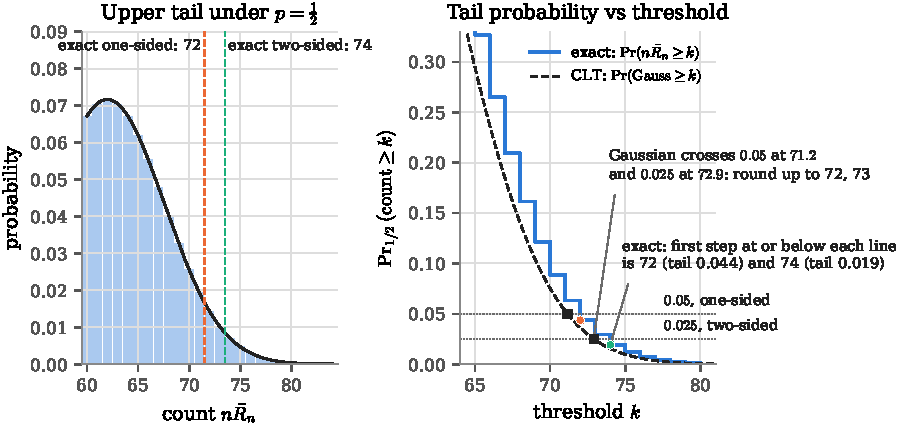
\includegraphics[width=\textwidth]{fig_exact_vs_clt}
\caption{Left: the upper tail of $\mathrm{Bin}(124, \frac12)$ (bars) and the $\Gauss(62, 31)$ density (curve), with the exact thresholds $72$ (orange) and $74$ (aqua) dashed. Right: $\Pr_{1/2}(\text{count} \geq k)$ against $k$, exact (staircase) and Gaussian (dashed), with the levels $0.05$ and $0.025$ dotted.}
\label{fig:exactclt}
\end{figure}

\textbf{Why they differ.}
\Cref{fig:exactclt} shows the two tail probabilities side by side.
On the left is the $\Gauss(62, 31)$ density the CLT puts in place of the $\mathrm{Bin}(124, \frac12)$ bars; on the right is the tail probability $\Pr_{1/2}(\text{count} \geq k)$ as a function of the threshold $k$, a staircase for the exact distribution and a smooth curve for the Gaussian.
The exact threshold is the first step at or below the level line, $72$ for $0.05$ and $74$ for $0.025$; the CLT threshold is where the curve crosses the line, $71.2$ and $72.9$, rounded up to $72$ and $73$.
The Gaussian curve is a good approximation of the staircase, off by about $0.005$ at $k = 73$, but $0.005$ is enough to put the exact tail ($0.029$) above the line $0.025$ and the Gaussian tail ($0.024$) below it, and that is the whole disagreement.
The gap is mostly discreteness, not the CLT's inaccuracy: the Gaussian approximates the probability of the count being $\geq 73$ better if the threshold is placed at $72.5$ (the \textbf{continuity correction} of an introductory course), and with it the two-sided threshold becomes $62 + 0.5 + 10.9 = 73.4$, rounding up to $74$, in agreement with the exact test.
This book does not use the correction. For a proportion, whenever the Gaussian approximation lands close enough to the line that the correction would change the decision, the exact Binomial test is available and settles the question outright. An asymptotic level $5\%$ is not an exact level $5\%$, and at a threshold where the exact tail is near the line the two can round in different directions.
For $80$ right turns, far from either threshold, the decision is the same every way: reject.

\begin{bridge}[the binomial test and the $z$-test for a proportion]
An introductory course presents these as two tests: the `exact binomial test' when $n$ is small, the `$z$-test for a proportion' when $np_0$ and $n(1 - p_0)$ are both at least $10$.
They test the same hypothesis with the same statistic, the count, and differ only in whether the count's distribution under $H_0$ is used as it is or replaced by its Gaussian limit.
The rule of thumb keeps the count's skewness small (the `$np \geq 10$' bridge in \cref{sec:clt}); it does nothing about discreteness, which is why the two-sided thresholds above still differ by one count with $np_0 = 62$.
\end{bridge}

\section{\texorpdfstring{$p$}{p}-values}
\label{sec:tests-pvalue}

A test as defined reports one bit, reject or not, at one level fixed in advance.
That loses information: a $T_n$ of $1.97$ and a $T_n$ of $3.23$ both reject at $5\%$, and the second is much stronger evidence.
It also forces the reader to accept the writer's $\alpha$.
The $p$-value fixes both.

\begin{definition}[$p$-value]
\label{def:pvalue}
Let $(\psi_\alpha)_{\alpha \in (0,1)}$ be a family of tests of $H_0$ indexed by their level, nested so that rejecting at level $\alpha$ implies rejecting at every level above $\alpha$.
The \textbf{(asymptotic) $p$-value} of the family on a given sample is the smallest (asymptotic) level $\alpha$ at which $\psi_\alpha$ rejects $H_0$ on that sample.\footnote{Strictly an infimum: at the boundary level the threshold equals the observed statistic and the strict inequality in $\psi_\alpha$ fails. The boundary case has probability zero, and the golden rule's $\leq$ settles it by convention.}
It is random: it depends on the sample.
\end{definition}

\begin{inwords}
\textbf{In words.} Run the test at every level at once. At large $\alpha$ it rejects easily, at small $\alpha$ it is hard to satisfy; the $p$-value is the level where it switches. Equivalently, for the standardized-mean tests of this chapter, it is the probability under $H_0$ of a test statistic at least as extreme as the one observed: the tail area beyond the observed value.
\par\smallskip
\textbf{For the kiss data.} $T_n = 3.23$. Two-sided, the $p$-value is $\Pr(\abs{Z} > 3.23) = 2(1 - \Phi(3.23)) = 0.0012$; one-sided, $\Pr(Z > 3.23) = 0.0006$. The exact Binomial tails give $0.0016$ and $0.0008$. Under $p = \frac12$, $80$ or more right turns out of $124$ is a one-in-a-thousand event.
\end{inwords}

\begin{figure}[htbp]
\centering
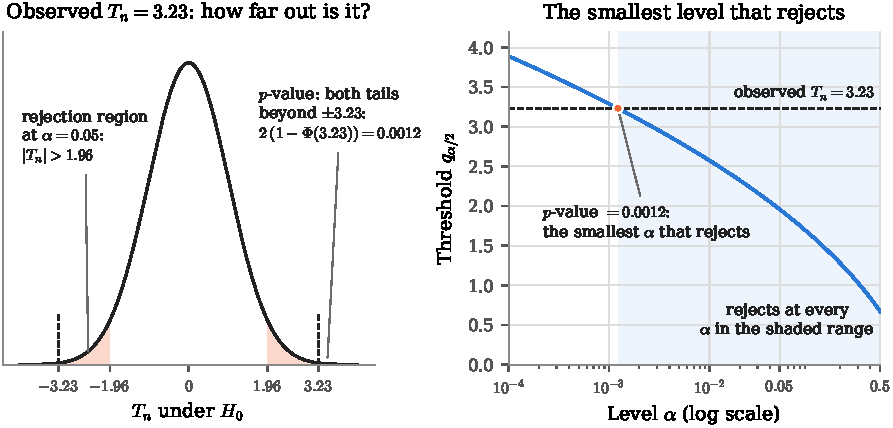
\includegraphics[width=\textwidth]{fig_pvalue}
\caption{The $p$-value for $T_n = 3.23$. Left: the density of $T_n$ under $H_0$, the rejection region at $5\%$ (light orange), the area beyond $\pm 3.23$ (dark orange), the observed value (dashed). Right: the threshold $q_{\alpha/2}$ against the level $\alpha$, with the observed value dashed.}
\label{fig:pvalue}
\end{figure}

\Cref{fig:pvalue} shows the $p$-value two ways.
On the left, the density of $T_n$ under $H_0$ is the standard Gaussian by the CLT, the $5\%$ rejection region is $\abs{T_n} > 1.96$, and the $p$-value is the area beyond $\pm 3.23$, too small to see at this scale: the probability under $H_0$ of something at least this extreme, $0.0012$.
On the right, the threshold $q_{\alpha/2}$ is drawn as a function of the level, with the observed value as a horizontal line; the test rejects at every level whose threshold lies below the line, and the smallest such level, where the curve crosses, is the $p$-value.
The two readings are the same number because of how the thresholds are built.
For the two-sided test, $\psi_\alpha$ rejects when $\abs{T_n} > q_{\alpha/2}$, and $q_{\alpha/2}$ decreases as $\alpha$ grows, so the levels at which the test rejects are exactly those with $q_{\alpha/2} < \abs{t}$ for the observed $t$, that is, those with $\alpha/2 > \Pr(Z > \abs{t})$, that is, $\alpha > \Pr(\abs{Z} > \abs{t})$.
The smallest such $\alpha$ is $\Pr(\abs{Z} > \abs{t})$, the tail area.
For a one-sided test with $H_1: \mu > \mu_0$ the same argument gives $\Pr(Z > t)$.
Since $\Pr(\abs{Z} > \abs{t}) = 2\Pr(Z > \abs{t})$, a two-sided $p$-value is twice the one-sided one when the data lean the alternative's way; when they lean the other way the one-sided $p$-value is above $\frac12$ and the one-sided test cannot reject. That is the one-sided test's advantage of \cref{sec:tests-clt} seen from the other end: it spends its whole $\alpha$ on one side and is blind to the other.

\textbf{The golden rule.}
The consequence of the definition is the rule worth memorizing:
\[
p\text{-value} \leq \alpha \quad \Longleftrightarrow \quad H_0 \text{ is rejected by } \psi_\alpha \text{ at (asymptotic) level } \alpha.
\]
So one number replaces the whole family of tests.
A reader who wants level $5\%$ compares the $p$-value with $0.05$; one who wants $1\%$ compares with $0.01$; and the smaller the $p$-value, the more levels reject, the more confidently $H_0$ is rejected.

\begin{bridge}[$p < 0.05$]
`Reject if $p < 0.05$' was the rule of an introductory course, and the golden rule is its justification: the $p$-value is the smallest level that rejects, so a $p$-value below $0.05$ means the level-$5\%$ test rejects, no more and no less.
Two habits from that course transfer intact. The $p$-value is computed from the null distribution of the statistic, which is why it needed $\mu_0$ (or $p_0$) and not any guess at the alternative. And a one-sided $p$-value is half the two-sided one for a symmetric statistic when the data lean the alternative's way, so the choice of sides made in \cref{sec:tests-hypotheses} before seeing the data is the choice that fixes the $p$-value.
\end{bridge}

\begin{pitfall}[what a $p$-value is not]
A $p$-value of $0.0012$ is the probability, computed as if $H_0$ were true, of data at least as extreme as these.
It is not the probability that $H_0$ is true; in this part of the book $H_0$ is true or false and has no probability (\cref{ch:bayes-intro} is where hypotheses get probabilities, and the number it produces is a different one).
It is not the probability that the result `was due to chance'.
And it is not a measure of the size of the effect: with $n$ large enough, a true $p$ of $0.51$ produces a tiny $p$-value (at $n = 100{,}000$, $T_n = 2\sqrt{n} \times 0.01 = 6.3$), since by \cref{prop:clt-test} the test detects any fixed departure eventually.
The $p$-value answers one question, how surprising the data would be under $H_0$, and the confidence interval of \cref{ch:confidence-intervals} answers the other, how big the departure is.
Report both.
\end{pitfall}

\begin{intuition}[the $p$-value is a statistic, and under $H_0$ it is uniform]
The $p$-value is a function of the sample, so it is a random variable, and it has a distribution under each $\theta$.
Under a simple $H_0$, for a test statistic with a continuous distribution, that distribution is uniform on $[0, 1]$: a $p$-value below $0.05$ happens $5\%$ of the time, below $0.01$ $1\%$ of the time, which is just the level restated (\cref{ex:tests-uniform} proves it).
Under $H_1$ the distribution piles up near $0$, and the more so the larger $n$.
So a small $p$-value is not proof; it is an event that is rare under $H_0$ and common under $H_1$.
\end{intuition}

\section{Tests and confidence intervals are one construction}
\label{sec:tests-duality}

\Cref{ex:ci-onesided} in \cref{ch:confidence-intervals} found that `$\frac12$ is below the conservative lower confidence bound' is the same event as `$n\bar{R}_n \geq 72$', the one-sided test's rejection.
That was not a coincidence of the kiss data.

\begin{proposition}[Duality of tests and confidence intervals]
\label{prop:duality}
Let $\Theta \subseteq \real$.
\begin{enumerate}[nosep]
\item Suppose that for every $\theta_0 \in \Theta$ there is a test $\psi(\theta_0)$ of $H_0: \theta = \theta_0$ with level $\alpha$.
Then the set of values not rejected,
\[
\mathcal{I} = \{ \theta_0 \in \Theta : \psi(\theta_0) = 0 \},
\]
is a confidence set of level $1 - \alpha$ for $\theta$.
\item Conversely, if $\mathcal{I}$ is a confidence interval of level $1 - \alpha$ for $\theta$, then for every $\theta_0$ the test $\psi(\theta_0) = \ind(\theta_0 \notin \mathcal{I})$ has level $\alpha$ for $H_0: \theta = \theta_0$.
\end{enumerate}
The same holds with `asymptotic' in front of both levels.
\end{proposition}

\coreproof{Both directions are one line: the event `the true $\theta$ is not in $\mathcal{I}$' is the event `the test of the true $\theta$ rejects', whose probability is the type 1 error.}
\begin{proof}
(1) For any true $\theta$, $\Pr_\theta(\mathcal{I} \not\ni \theta) = \Pr_\theta(\psi(\theta) = 1) = \alpha_{\psi(\theta)}(\theta) \leq \alpha$, since $\psi(\theta)$ has level $\alpha$ for the null $\theta = \theta$, which is true.
So $\Pr_\theta(\mathcal{I} \ni \theta) \geq 1 - \alpha$ for every $\theta$: the coverage condition of \cref{def:ci}, applied to a set rather than an interval.
(2) Under $H_0: \theta = \theta_0$ the truth is $\theta_0$, and $\Pr_{\theta_0}(\psi(\theta_0) = 1) = \Pr_{\theta_0}(\mathcal{I} \not\ni \theta_0) \leq \alpha$ by the coverage guarantee.
The asymptotic version replaces each probability by its limit.
\end{proof}

\begin{figure}[htbp]
\centering
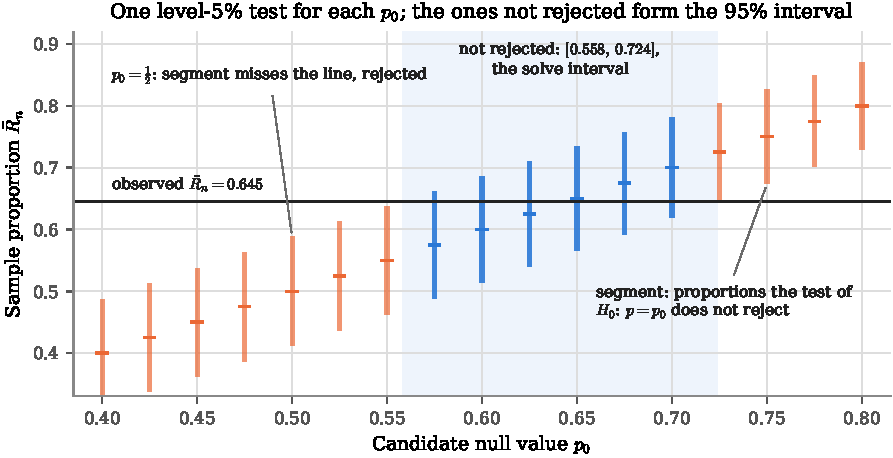
\includegraphics[width=\textwidth]{fig_test_ci_duality}
\caption{The duality for the kiss data. At each candidate $p_0$ (horizontal axis), a vertical segment $p_0 \pm 1.96\sqrt{p_0(1-p_0)/124}$; the horizontal line is the observed $\bar{R}_n = 0.645$. Segments crossing the line are blue, segments missing it are orange, and the shaded strip is $[0.558, 0.724]$.}
\label{fig:duality}
\end{figure}

\Cref{fig:duality} draws part (1) for the kiss data, running the test for every $p_0$ at once.
Each vertical segment is the set of sample proportions the level-$5\%$ test of $H_0: p = p_0$ does not reject; a candidate whose segment crosses the line of the observed $\bar{R}_n = 0.645$ is not rejected, one whose segment misses it is rejected, and $\frac12$ misses.
The shaded strip of candidates not rejected is $[0.558, 0.724]$, the solve interval of \cref{ch:confidence-intervals} exactly.
The test being inverted is
\[
\psi(p_0) = \ind\left\{ \abs{\bar{R}_n - p_0} > q_{\alpha/2}\sqrt{p_0(1 - p_0)/n} \right\},
\]
which measures the distance from $p_0$ in units of the standard error computed \textit{at $p_0$}, the value the null hypothesis asserts. For a proportion, a test built that way, from the standard error under the null rather than from an estimate, is the \textbf{score test}, which \cref{ch:wald-lrt} defines for any model.
The candidates that survive are those with $\abs{\bar{R}_n - p_0} \leq q_{\alpha/2}\sqrt{p_0(1-p_0)/n}$, which is the inequality that \cref{sec:ci-three-solutions} solved to get the solve interval $[0.558, 0.724]$.
So the solve interval is the set of null values the score test does not reject, and the score test of $p = \frac12$ rejects exactly because $\frac12$ is outside the interval. This is why \cref{sec:ci-three-solutions} called the result the Wilson score interval: it is the score test, inverted.
Inverting the test built from the \textit{estimated} standard error $\sqrt{\bar{R}_n(1 - \bar{R}_n)/n}$ instead gives the plug-in interval $[0.561, 0.729]$. That one is \textbf{Wald's test}, which \cref{ch:wald-lrt} treats in general. Score and Wald are the same idea evaluated at two different places, the null value and the estimate, and they are the two tests you will meet most often.
And the one-sided test of \cref{ex:ci-onesided} inverts to a one-sided interval, a lower confidence bound.
Every interval in \cref{ch:confidence-intervals} is a test turned inside out, and every test here is an interval asked about one point.

\begin{bridge}[if the confidence interval excludes the null value, reject]
An introductory course states this as a shortcut: `the $95\%$ confidence interval is $[0.56, 0.73]$, which does not contain $0.5$, so the difference is significant at $5\%$'.
\Cref{prop:duality} is why the shortcut is legitimate, and it also says when it is exact and when it is approximate.
The shortcut reproduces the test's decision exactly when the test and the interval are built from the same standard error, the solve interval for the score test and the plug-in interval for Wald's, and only approximately otherwise.
Using the plug-in interval to decide a score test can disagree with it on a borderline sample, since the two standard errors differ: $\sqrt{\bar{R}_n(1 - \bar{R}_n)/n} = 0.043$ against $\sqrt{\frac12 \cdot \frac12 / n} = 1/(2\sqrt{n}) = 0.045$ here. Far from the border, as with $80$ picks, every version agrees.
\end{bridge}

\section{What comes next}
\label{sec:tests-next}

This chapter built one test, the standardized mean against a Gaussian quantile, and the ideas that describe any test.
The remaining tests in this book are the same object with a different statistic and a different null distribution.
\Cref{ch:t-test} replaces the Gaussian quantile by a Student quantile when $n$ is small and the data are Gaussian, which needs the chi-squared distribution and Cochran's theorem for the sample variance; it also finishes the boarding example as a two-sample test.
\Cref{ch:wald-lrt} gives three general recipes for a test statistic in any parametric model, Wald's test (the standardized maximum likelihood estimator), the likelihood ratio test and the score test, with chi-squared limits in place of Gaussian ones.
\Cref{ch:gof} and \cref{ch:ks} test the model itself rather than a parameter in it, with the same vocabulary: a statistic, a null distribution, a threshold, a $p$-value.
In all of them the level is the cap on the type 1 error, the power is what the test can detect, and the $p$-value is what gets reported.

\section{Summary}
\label{sec:tests-summary}

\begin{itemize}[nosep]
\item Hypotheses: $H_0: \theta \in \Theta_0$ against $H_1: \theta \in \Theta_1$, disjoint. The data are used only to try to reject $H_0$; failing to reject is not accepting. Simple ($\{\theta_0\}$) or composite; one-sided or two-sided, and the side is chosen before the data are seen.
\item A test is $\psi: E^n \to \{0,1\}$, the indicator of its rejection region; in practice $\psi = \ind(T_n > c)$ for a test statistic $T_n$ and a threshold $c$.
\item Type 1 error $\alpha_\psi(\theta) = \Pr_\theta(\psi = 1)$ on $\Theta_0$; type 2 error $\beta_\psi(\theta) = \Pr_\theta(\psi = 0)$ on $\Theta_1$; power $\pi_\psi = \inf_{\Theta_1}(1 - \beta_\psi)$. At fixed $n$ the two errors trade off; only $n$ lowers both.
\item Level $\alpha$: $\alpha_\psi \leq \alpha$ on all of $\Theta_0$, a cap on the worst case; asymptotic level: the same in the limit. For a composite null the worst case is at the boundary, so $H_0: \theta \leq \theta_0$ and $H_0: \theta = \theta_0$ get the same test. For a test the level is $\alpha$; for an interval it is $1 - \alpha$.
\item The standardized-mean test: $T_n = \sqrt{n}(\bar{X}_n - \mu_0)/\sigma$, reject if $\abs{T_n} > q_{\alpha/2}$ (two-sided) or $T_n > q_\alpha$ (one-sided). Asymptotic level $\alpha$ by the CLT, plus Slutsky if $\sigma$ is estimated; consistent (power $\to 1$ at every fixed alternative) by the LLN. Under $H_0$ the parameter is known, so no plug-in is needed.
\item Kiss experiment: $T_n = 3.23$, reject at $5\%$ either way. Exact Binomial thresholds $72$ (one-sided) and $74$ (two-sided); CLT thresholds $72$ and $73$. They differ because the exact tail is a staircase and $0.025$ falls between two of its steps.
\item $p$-value: the smallest level at which the data reject; for these tests, the tail area beyond the observed statistic under $H_0$. Golden rule: $p$-value $\leq \alpha$ if and only if $\psi_\alpha$ rejects. Kiss experiment: $0.0012$ two-sided, $0.0006$ one-sided. Not the probability that $H_0$ is true.
\item Duality: the null values a level-$\alpha$ test does not reject form a level-$(1-\alpha)$ confidence set, and a level-$(1-\alpha)$ interval rejects every null value outside it at level $\alpha$. The solve interval inverts the score test, which uses the standard error at the null value; the plug-in interval inverts Wald's test, which uses the estimated standard error.
\end{itemize}

\section{Exercises}
\label{sec:tests-exercises}

\begin{exercise}
\label{ex:tests-kiss-pvalue}
For $80$ of $124$ couples turning right, formulate the two-sided hypothesis problem, compute the $p$-value by the CLT and exactly, and conclude. Then do the one-sided version.
\end{exercise}
\begin{solution}
$H_0: p = \frac12$ against $H_1: p \neq \frac12$ in the model $(\{0,1\}, (\Bern(p))_{p \in (0,1)})$. $T_n = 2\sqrt{124}(0.6452 - 0.5) = 3.23$. CLT $p$-value: $2(1 - \Phi(3.23)) = 0.0012$. Exact: $\Pr_{1/2}(n\bar{R}_n \geq 80) = 0.0008$, doubled for two sides, $0.0016$. Both are far below $0.05$ (and below $0.01$): reject $H_0$ at any conventional level; the data are not compatible with equal appeal. One-sided, $H_1: p > \frac12$: $p$-values $1 - \Phi(3.23) = 0.0006$ (CLT) and $0.0008$ (exact), half the two-sided ones.
\end{solution}

\begin{exercise}
\label{ex:tests-cookies}
(From OpenIntro Statistics.) Students count the chocolate chips in $32$ cookies and find a mean of $14.77$ with a standard deviation of $4.37$. The packaging claims at least $20$ chips per cookie. One student says the claim is unreasonable; another says the difference might be chance. Formulate the hypotheses, compute a $p$-value and decide, saying what approximation you used.
\end{exercise}
\begin{solution}
Let $\mu$ be the mean number of chips. The claim is the null, $H_0: \mu \geq 20$, and the student's doubt is the alternative, $H_1: \mu < 20$: a one-sided test with the threshold computed at the boundary $\mu_0 = 20$. With $\sigma$ replaced by the sample standard deviation, $T_n = \sqrt{32}\,(14.77 - 20)/4.37 = -6.77$. By the CLT and Slutsky the $p$-value is approximately $\Phi(-6.77) \approx 6 \times 10^{-12}$: reject at every conventional level; the difference is not chance. The approximation is the Gaussian limit at $n = 32$ with an estimated $\sigma$; \cref{ch:t-test} replaces it by Student's $t$ with $31$ degrees of freedom, for which $-6.77$ is just as decisive.
\end{solution}

\begin{exercise}
\label{ex:tests-cancer}
A machine learning procedure claims to reduce the rate of surgery on benign tumors below the state of the art, $95\%$, while keeping the true positive rate. On $297$ benign tumors it recommended surgery for $206$. Let $p$ be the proportion of benign tumors on which it prescribes surgery. Formulate the hypotheses, compute the $p$-value and conclude.
\end{exercise}
\begin{solution}
The claim needs evidence, so it is the alternative: $H_0: p \geq 0.95$ against $H_1: p < 0.95$, one-sided, threshold at the boundary $p_0 = 0.95$. $\hat{p} = 206/297 = 0.6936$ and $T_n = \sqrt{297}\,(0.6936 - 0.95)/\sqrt{0.95 \times 0.05} = -20.3$. The $p$-value $\Phi(-20.3)$ is zero to every decimal place anyone prints: reject $H_0$; the procedure's false positive rate is below $95\%$. (Whether it is below by enough to matter is the confidence interval's question: $0.694 \pm 1.96\sqrt{0.694 \times 0.306/297} = [0.64, 0.75]$.)
\end{solution}

\begin{exercise}
\label{ex:tests-coin}
For the fair coin ($13$ heads in $30$ tosses), compute the two-sided $p$-value by the CLT and exactly, and comment on the gap.
\end{exercise}
\begin{solution}
$T_n = -0.73$, CLT $p$-value $2\Phi(-0.73) = 0.47$. Exactly, $\Pr_{1/2}(\mathrm{Bin}(30, \frac12) \leq 13) = 0.292$, doubled $0.58$. Neither is close to rejecting. The gap between $0.47$ and $0.58$ is the discreteness of \cref{fig:exactclt} at $n = 30$: the Gaussian tail beyond $13$ undercounts the mass of the bar at $13$ itself, which the continuity correction (evaluating at $13.5$) largely repairs: $2\Phi(\sqrt{30}(13.5/30 - 0.5)/0.5) = 2\Phi(-0.55) = 0.58$.
\end{solution}

\begin{exercise}
\label{ex:tests-interval-null}
For $\Xton \iid \Pois(\lambda)$, build a test of asymptotic level $5\%$ for $H_0: \abs{\lambda - 2} \leq 1$ against $H_1: \abs{\lambda - 2} > 1$.
\end{exercise}
\begin{solution}
$\Theta_0 = [1, 3]$. Reject when $\hat{\lambda}$ is far outside it on either side, with a margin that shrinks like $1/\sqrt{n}$ and uses the standard deviation $\sqrt{\lambda}$ at its own endpoint: $\psi = \ind(\hat{\lambda} > 3 + s\sqrt{3/n}) + \ind(\hat{\lambda} < 1 - s\sqrt{1/n})$ for a number $s$ to be chosen (the two events are disjoint, since $\hat{\lambda}$ cannot be both above $3$ and below $1$). The type 1 error at $\lambda \in [1, 3]$ is largest at the endpoints: at $\lambda = 3$ the first indicator is the event $\sqrt{n}(\hat{\lambda} - 3)/\sqrt{3} > s$, whose probability tends to $\Pr(Z > s)$ by the CLT, and the second indicator's probability tends to $0$ by the LLN; at $\lambda = 1$ the reverse, with limit $\Pr(Z < -s)$. At any interior $\lambda$ both probabilities tend to $0$. Choosing $s = 1.645$ makes each endpoint's limiting type 1 error $0.05$, so the test has asymptotic level $5\%$ (not $2.5\%$ per side: at any one $\lambda$ only one side can fire in the limit). Each side uses the standard deviation $\sqrt{\lambda}$ at its own endpoint, which is the `parameter known under the null' idea applied endpoint by endpoint.
\end{solution}

\begin{exercise}
\label{ex:tests-uniform}
Let $T$ be a test statistic with a continuous, strictly increasing CDF $F_0$ under $H_0$, and let the test reject for large $T$, so the $p$-value is $P = 1 - F_0(T)$. Show that under $H_0$, $P$ is uniform on $[0, 1]$, and deduce that $\Pr_{H_0}(P \leq \alpha) = \alpha$ for every $\alpha$: the golden rule gives exact level $\alpha$.
\end{exercise}
\begin{solution}
For $u \in (0, 1)$, $\Pr_{H_0}(P \leq u) = \Pr_{H_0}(1 - F_0(T) \leq u) = \Pr_{H_0}(F_0(T) \geq 1 - u) = \Pr_{H_0}(T \geq F_0^{-1}(1 - u)) = 1 - F_0(F_0^{-1}(1 - u)) = u$, using that $F_0$ is continuous and strictly increasing so that $F_0^{-1}$ exists and $\Pr(T = t) = 0$ \toolkit{sec:math-density}. A CDF equal to $u$ on $(0,1)$ is the uniform CDF. Then $\Pr_{H_0}(P \leq \alpha) = \alpha$, which is the golden rule's `reject when $P \leq \alpha$' having type 1 error exactly $\alpha$. For a discrete $T$ the equality becomes $\leq \alpha$, the staircase of \cref{sec:tests-kiss}.
\end{solution}

\begin{exercise}
\label{ex:tests-solve-inversion}
Show that the set of $p_0 \in (0,1)$ not rejected by the test $\psi(p_0) = \ind(\abs{\bar{R}_n - p_0} > q_{\alpha/2}\sqrt{p_0(1 - p_0)/n})$ is exactly the solve interval of \cref{sec:ci-three-solutions}, and that inverting the test with the plug-in standard error gives the plug-in interval.
\end{exercise}
\begin{solution}
Not rejecting $p_0$ means $\abs{\bar{R}_n - p_0} \leq q_{\alpha/2}\sqrt{p_0(1-p_0)/n}$, that is, $(\bar{R}_n - p_0)^2 \leq q_{\alpha/2}^2\, p_0(1 - p_0)/n$, the quadratic inequality in $p_0$ whose solution set is the solve interval (\cref{eq:wilson}). With $\sqrt{\bar{R}_n(1 - \bar{R}_n)/n}$ in place of $\sqrt{p_0(1-p_0)/n}$ the inequality is $\abs{\bar{R}_n - p_0} \leq q_{\alpha/2}\sqrt{\bar{R}_n(1 - \bar{R}_n)/n}$, whose solution set is $\bar{R}_n \pm q_{\alpha/2}\sqrt{\bar{R}_n(1-\bar{R}_n)/n}$, the plug-in interval. The conservative interval inverts the test that uses the worst-case standard error $1/(2\sqrt{n})$ for every $p_0$.
\end{solution}
